% =====================================================================
% Seminar S04 report: LIME and SHAP (English version)
% Compile with XeLaTeX (Overleaf: Menu -> Compiler -> XeLaTeX)
% Figures are in the figs_en/ folder
% =====================================================================
\documentclass[11pt,a4paper]{article}
\usepackage[a4paper,margin=2.0cm]{geometry}
\emergencystretch=2em
\usepackage{fontspec}
\usepackage{amsmath,amssymb}
\usepackage{booktabs,tabularx,array}
\usepackage{graphicx}
\usepackage{float}
\usepackage[font=small,labelfont=bf]{caption}
\usepackage{enumitem}
\usepackage{pgfplots}
\usepackage[en-GB]{datetime2}
\pgfplotsset{compat=1.16}
\usepackage[colorlinks=true,linkcolor=black,urlcolor=blue,citecolor=black]{hyperref}

\setlist{itemsep=2pt,topsep=3pt,parsep=0pt}
\setlength{\parindent}{0pt}
\setlength{\parskip}{5pt}
\renewcommand{\arraystretch}{1.15}
\newcolumntype{L}[1]{>{\raggedright\arraybackslash}p{#1}}
\newcommand{\code}[1]{\texttt{#1}}
\newcommand{\coderepo}{\href{https://github.com/khoiLearnsToCode/CS420_AI_LIME_SHAP}{code repository}}

\title{\textbf{LIME and SHAP: Explaining Machine-Learning Predictions}\\[2pt]\large Seminar S04 Report -- CS420}
\author{%
  Nguyễn Trọng Hoàng\\ \small 24125056 \and
  Phan Minh Khôi\\ \small 24125061 \and
  Nguyễn Thuận Việt\\ \small 24125051%
}
\date{}

\begin{document}
\maketitle

\begin{abstract}
Machine-learning models are increasingly used in high-stakes fields such as
medicine, yet a model that is usually right does not automatically reveal why
it made a particular decision. This report asks whether a highly accurate
prediction necessarily comes with a reliable explanation, focusing on two
widely used tools, LIME (Local Interpretable Model-agnostic Explanations) and
SHAP (SHapley Additive exPlanations), which estimate how much each input
feature contributed to a single prediction. We apply both tools to two models
trained to detect breast cancer from tumour measurements and examine an easy,
a borderline and a misclassified case, asking whether the tools agree, whether
their results stay the same when re-run, and whether the features they rank
highest truly drive the prediction. Although the models are 98.2\% and 95.6\%
accurate, the tools agree well only on the easy case: on the misclassified
case they share just two of their five most important features, and their
rankings shift noticeably between runs. Both tools find influential features
far better than random choice, but neither is clearly more reliable than the
other. We therefore recommend repeating explanations and checking their
stability before trusting them, especially for uncertain or incorrect
predictions.
\end{abstract}

%---------------------------------------------------------------------
\section{Introduction}

Many modern machine-learning models are ``black boxes'': we see the input and
the output but not which features drive a decision. In healthcare, finance or
autonomous driving, a prediction cannot be trusted just because it is usually
right, so the need to explain individual decisions keeps growing
\cite{ribeiro}\cite{mersha}. LIME \cite{ribeiro} and SHAP \cite{lundberg} are
two widely used post-hoc methods for this purpose.

\paragraph{Guiding question.} Does a highly accurate prediction necessarily
come with a reliable explanation? To answer it, we look at three
criteria: whether an explanation is useful (it shows which features push the
prediction up or down), stable (it does not change with the seed or the
background data) and faithful to the model (removing features called important
should change the prediction accordingly).

\paragraph{Scope.} We use the Breast Cancer Wisconsin dataset \cite{street}
(569 instances, 30 features, two classes), two models (Logistic Regression and
Random Forest) and three instances chosen by a fixed rule. The two source
papers are Ribeiro et al.~\cite{ribeiro} for LIME and Lundberg \&
Lee~\cite{lundberg} for SHAP; the survey by Mersha et al.~\cite{mersha} is used
to place both methods in the XAI taxonomy and to choose evaluation criteria.

\paragraph{Contributions.} We (i) synthesise and compare the two required
papers \cite{ribeiro}\cite{lundberg} and one survey \cite{mersha}; (ii) work
through SHAP on a linear model and LIME on a small non-linear model by hand;
(iii) compare the two methods on top-$k$ overlap, runtime and stability across
seeds and background sets; and (iv) run a deletion test and propose a
procedure for evaluating faithfulness. What belongs to the papers carries a
citation; the remaining examples and numbers are our own.
%---------------------------------------------------------------------
\section{Background and Paper Review}

\subsection{Core concepts}
Mersha et al.~\cite{mersha} point out that the terminology of XAI is not yet
settled. In this report, \emph{interpretability} means how well a person can
understand how a model works internally, and \emph{explainability} means the
ability to give reasons for \emph{one specific decision}. Some authors treat one
term as a subset of the other, so we state our definitions explicitly.
Table~\ref{tab:concepts} lists the concept pairs used in the rest of the report
and shows where LIME and SHAP fall.

\begin{table}[!htb]
\centering\small
\caption{Core concept pairs and where LIME and SHAP fall.}\label{tab:concepts}
\begin{tabularx}{\textwidth}{L{3.3cm}XX}
\toprule
\textbf{Concept pair} & \textbf{Distinction} & \textbf{LIME and SHAP}\\
\midrule
Explainability -- interpretability & Explaining one prediction vs.\ understanding how the model works overall & Provide explainability; do not make the model interpretable\\
Local -- global & Explaining one instance vs.\ describing the whole model & Both are local; LIME adds SP-LIME to pick representative instances for a global view \cite{ribeiro}\\
Model-specific -- model-agnostic & Depends on model structure vs.\ needs only the prediction function & LIME and KernelSHAP are model-agnostic; Linear SHAP and Deep SHAP are model-specific \cite{lundberg}\\
Intrinsic (ante-hoc) -- post-hoc & Model is understandable by design vs.\ explained after training & Both are post-hoc and perturbation-based \cite{mersha}\\
\bottomrule
\end{tabularx}
\end{table}

\subsection{LIME}\label{sec:lime}
LIME, proposed by Ribeiro et al.~\cite{ribeiro}, explains a single prediction by
fitting a simple model that imitates the black box near the instance of
interest. It samples perturbed points around an input $x$, queries the
black-box model at each point, and fits an interpretable surrogate in which
points closer to $x$ count more. Formally, the explanation is
\begin{equation}\label{eq:lime}
\xi(x) = \arg\min_{g \in G} \; L(f, g, \pi_x) + \Omega(g),
\end{equation}
\begin{equation}\label{eq:limeloss}
L(f, g, \pi_x) = \sum_{z, z'} \pi_x(z) \big( f(z) - g(z') \big)^2, \qquad \pi_x(z) = \exp\!\big( -D(x, z)^2 / \sigma^2 \big).
\end{equation}
Here $f$ is the black-box model; in our experiments $f(x) \in [0,1]$ is the
predicted probability of one class. $x \in \mathbb{R}^d$ is the instance being
explained ($d = 30$ in our data), $z \in \mathbb{R}^d$ is a perturbed sample in
the original feature space, and $z' \in \{0,1\}^N$ is its interpretable
representation over $N$ interpretable components, where $z'_i = 1$ if the
$i$-th component is present in $z$ and $z'_i = 0$ otherwise. $G$ is a family of
interpretable models (here linear models $g(z') = w_g \cdot z'$), $D \geq 0$ is
a distance function (Euclidean in our worked example) and $\sigma > 0$ is the
kernel width, so $\pi_x(z) \in (0, 1]$ and $L \geq 0$ is measured in squared
probability units. $\xi(x)$ is the chosen surrogate, whose weights $w_g$ are
the explanation.

Two terms in Eq.~\eqref{eq:lime} shape the explanation:
\begin{itemize}
  \item The proximity kernel $\pi_x(z)$ defines what ``local'' means: the closer
        a perturbed sample is to $x$, the more weight it receives. The kernel
        width $\sigma$ sets the size of this neighbourhood. If $\sigma$ is too
        small, only a few samples carry meaningful weight and the explanation
        becomes noisy; if it is too large, the surrogate is no longer local.
  \item The complexity penalty $\Omega(g)$ keeps the explanation short. For
        linear surrogates Ribeiro et al.\ set
        $\Omega(g) = \infty \cdot \mathbb{1}\big[\lVert w_g \rVert_0 > K\big]$,
        which forbids more than $K$ non-zero weights, and use K-LASSO to
        select the $K$ features to keep. This trades some local fidelity for
        readability.
\end{itemize}
% Implementation note: the \code{lime} library for tabular data discretises continuous features by default, so a LIME weight is the effect of the value range the instance falls into, not a contribution relative to a baseline as in SHAP.

\subsection{SHAP}
\label{sec:shap}
SHAP, introduced by Lundberg and Lee~\cite{lundberg}, starts from a class of
methods the authors call \emph{additive feature attribution} methods. In this
class, the explanation model is a linear function of binary variables:
\begin{equation}
g(z') = \varphi_0 + \sum_{j=1}^{M} \varphi_j z'_j, \qquad z' \in \{0, 1\}^M,
\end{equation}
where $\varphi_j$ is the attribution of feature $j$ and $M$ is the number of
features ($M = 30$ in our data). The attributions have the same unit as $f$:
in our experiments $\varphi_0 \in [0, 1]$ and each $\varphi_j \in [-1, 1]$ is
a change in probability. The authors prove (Theorem~1) that only one choice of
attributions in this class satisfies three properties:
\begin{itemize}
  \item \emph{local accuracy}: the explanation reproduces the prediction,
        $g(x') = f(x)$;
  \item \emph{missingness}: a feature that is absent receives no attribution;
  \item \emph{consistency}: if the model changes so that a feature's marginal
        contribution does not decrease, its attribution does not decrease
        either.
\end{itemize}
This unique solution is the Shapley value:
\begin{equation}
\varphi_j = \sum_{S \subseteq F \setminus \{j\}} \frac{|S|! \, (M - |S| - 1)!}{M!} \Big[ f_{S \cup \{j\}}(x_{S \cup \{j\}}) - f_S(x_S) \Big].
\end{equation}
Here $F$ is the set of all $M$ features, $S$ is a subset that does not contain
feature $j$, and $f_S$ is the prediction when only the features in $S$ are
known; the remaining features are averaged out over a set of background data.
Three quantities matter when reading a SHAP explanation:
\begin{itemize}
  \item \textbf{Baseline.} $\varphi_0 = \mathbb{E}[f(X)]$ is the average
        prediction over the background data, so it depends on how that data is
        chosen.
  \item \textbf{Contribution.} $\varphi_j$ is the share of the gap between
        $f(x)$ and the baseline that feature $j$ accounts for; together,
        $\varphi_0 + \sum_j \varphi_j = f(x)$ exactly.
  \item \textbf{Sign.} A positive $\varphi_j$ pushes the prediction above the
        baseline, and a negative one pushes it below.
\end{itemize}
KernelSHAP estimates Shapley values with a weighted linear regression. Lundberg
and Lee show that this is LIME with a specific choice of kernel, loss and
regulariser (Theorem~2), and they note that LIME's heuristic choices of these
components can violate local accuracy or consistency. The estimation usually
assumes that features are independent, and some variants also assume that the
model is linear. For a linear model with independent features, the Shapley
values have the closed form $\varphi_j = w_j (x_j - \mathbb{E}[X_j])$, which is
the basis of the worked example in Section~\ref{sec:shaphand}.

\subsection{The survey by Mersha et al.}
Mersha et al.~\cite{mersha} classify XAI techniques along four axes: scope
(local or global), stage (ante-hoc or post-hoc), applicability (model-specific
or model-agnostic) and design methodology (perturbation-based or
gradient-based). To evaluate explanations, they separate human-centred
approaches from computer-centred ones and list five computer-centred criteria:
fidelity, consistency, robustness, efficiency and sufficiency. They also stress
that no single metric suits every system. We use these criteria to organise
the evaluation in Section~\ref{sec:results}.

\subsection{Comparing the three sources}
Table~\ref{tab:sources} compares the goal, main contribution and limitations
of the three sources.

\begin{table}[!htb]
\centering\small
\caption{Comparison of the three main sources.}\label{tab:sources}
\begin{tabularx}{\textwidth}{L{3.0cm}XXX}
\toprule
\textbf{Source} & \textbf{Goal} & \textbf{Main contribution} & \textbf{Limitations / notes}\\
\midrule
Ribeiro et al.~\cite{ribeiro} & Explain the predictions of any classifier so that people can decide whether to trust it & LIME (a sparse, locally weighted surrogate) and SP-LIME for picking representative instances & Kernel and $\sigma$ are chosen heuristically; no Shapley-style guarantees\\
Lundberg \& Lee~\cite{lundberg} & Unify existing feature-attribution methods & The additive attribution class, its unique solution (Shapley values) and KernelSHAP & Estimation assumes feature independence; results depend on the background data\\
Mersha et al.~\cite{mersha} & Survey XAI: taxonomy, applications and evaluation & A four-axis taxonomy and five evaluation criteria & Covers LIME and SHAP only briefly; we use its criteria in spirit, not its exact formulas (Section~\ref{sec:proc})\\
\bottomrule
\end{tabularx}
\end{table}

%---------------------------------------------------------------------
\section{Method and Worked Examples}
We describe the setup, then work through one small example per method so that
the computations behind Section~\ref{sec:results} can be followed.
\subsection{Experimental setup}
We use the Breast Cancer Wisconsin data \cite{street} from scikit-learn
(class 0 = malignant), an 80/20 stratified split (455 train, 114 test), a
standardised Logistic Regression (LR) and a 200-tree Random Forest (RF), with
test accuracy 98.2\% and 95.6\%. Both methods explain $P(\text{malignant})$:
SHAP with KernelSHAP (100 background instances, 2000 coalitions), LIME with
the library defaults (5000 samples, kernel width $\approx 4.11$). Every choice
was fixed before looking at the results and all seeds are fixed;
Appendix~\ref{app:setup} gives the full setup and the reason for each choice.

\textbf{Features.} The 30 features are computed from a digitised image of a
fine-needle aspirate: ten cell-nucleus measurements (radius, texture,
perimeter, area, smoothness, compactness, concavity, concave points, symmetry,
fractal dimension), each given as the mean, the standard error (``error'') and
the mean of the three largest values (``worst''). All values are non-negative
and no physical unit is given in the data: the size features are on the image
scale (area in squared units of radius) and the others are dimensionless
ratios or grey-level statistics. Their ranges differ widely, for example mean
radius $6.98$--$28.11$, worst area $185$--$4254$ and mean smoothness
$0.053$--$0.163$, which is why LR uses standardised inputs.

\textbf{Instances.} A fixed rule applied to the RF picks three test instances
(Table~\ref{tab:instances}): the correct prediction with the highest
confidence, the prediction with the smallest $|P - 0.5|$ and the first
misclassified one. This prevents us from choosing favourable examples.

\begin{table}[!htb]
\centering\small
\caption{The three chosen instances. $P > 0.5$ means the model predicts malignant.}\label{tab:instances}
\begin{tabular}{lccc}
\toprule
\textbf{Instance} & \textbf{Test index} & \textbf{True label} & \textbf{$P$(malignant), RF / LR}\\
\midrule
Confidently correct & 0 & malignant & 1.000 / 1.000\\
Borderline & 16 & benign & 0.495 / 0.634 (LR is wrong)\\
Misclassified & 3 & benign & 0.745 (RF is wrong) / 0.466\\
\bottomrule
\end{tabular}
\end{table}

\subsection{Worked example 1: SHAP on a linear model}\label{sec:shaphand}
Before applying SHAP to real data, we compute it by hand on a small linear
model to show how the baseline and the feature contributions are obtained and
to check that they add up to the prediction (local accuracy, Section~\ref{sec:shap}).
Assume the model $f(x) = b + \sum_j w_j x_j$, independent features, and the background is the mean $\mu_j = \mathbb{E}[X_j]$. Then $\varphi_0 = f(\mu)$ and $\varphi_j = w_j (x_j - \mu_j)$. Take $b = 1$, $w = (2, -1, 0.5)$, $\mu = (1, 2, 4)$ and the instance $x = (3, 1, 6)$.
\begin{itemize}
  \item Baseline: $\varphi_0 = f(\mu) = 1 + 2\cdot 1 - 1\cdot 2 + 0.5\cdot 4 = 3$.
  \item Prediction: $f(x) = 1 + 2\cdot 3 - 1\cdot 1 + 0.5\cdot 6 = 9$.
  \item Contributions: $\varphi_1 = 2(3 - 1) = 4$; $\varphi_2 = (-1)(1 - 2) = 1$; $\varphi_3 = 0.5(6 - 4) = 1$.
  \item Check: $\varphi_0 + \varphi_1 + \varphi_2 + \varphi_3 = 3 + 4 + 1 + 1 = 9 = f(x)$.
\end{itemize}
Enumerating every subset with the original Shapley formula (with $v(S) = f$ where features in $S$ take their value from $x$ and the rest take the mean) gives the same result $(4, 1, 1)$. Feature 2 has $w_2 < 0$ but $x_2 < \mu_2$, so its contribution is still positive: the sign of $\varphi_j$ depends on both the coefficient and where the instance lies relative to the background.

\subsection{Worked example 2: LIME step by step}\label{sec:limehand}
We now run LIME by hand on a small non-linear model to show its three steps
(perturbing the input, weighting the samples by distance, and fitting a
weighted linear surrogate) and to compare the resulting coefficients with the
model's true local slopes.

\paragraph{Model and instance.} We use the model
\begin{equation}
f(x) = \operatorname{sigmoid}(x_1^2 - x_2), \qquad
\operatorname{sigmoid}(t) = \frac{1}{1 + e^{-t}}.
\end{equation}
The sigmoid function maps any real number $t$ to a value between 0 and 1, so
$f(x)$ can be read as a probability, as in logistic regression. The model is non-linear in its inputs, both because of the sigmoid and because
of the $x_1^2$ term, so a linear surrogate can only approximate it locally. The instance to explain is $x_0 = (1, 2)$, for which
$f(x_0) = \operatorname{sigmoid}(1 - 2) = \operatorname{sigmoid}(-1) = 0.2689$.

To keep the example traceable, we make three simplifications: we use 6 fixed
perturbed points instead of random sampling, set the kernel width to
$\sigma = 1$, and drop the complexity penalty $\Omega$. We also use the
original features (shifted by $x_0$) as the interpretable representation
instead of the binary vector $z'$ of Section~\ref{sec:lime}, so the coefficients can be
compared directly with the slopes of $f$.

\paragraph{Step 1: perturb and query.} For each perturbed point $z$, compute
the model output $f(z)$. For example, for $z = (1.3,\, 2.2)$ we get
$f(z) = \operatorname{sigmoid}(z_1^2 - z_2) =  \operatorname{sigmoid}(-0.51) = 0.3752$.

\paragraph{Step 2: weight by distance.} Compute the distance
$D = \lVert z - x_0 \rVert$ and the weight $\pi = \exp(-D^2/\sigma^2)$. For
$z = (1.3,\, 2.2)$, $D = \sqrt{(1.3 - 1)^2 +(2.2 - 2)^2} = 0.361$ and $\pi = 0.878$.
Points closer to $x_0$ receive weights closer to 1. Table~\ref{tab:limepoints}
lists all six points.

\begin{table}[!htb]
\centering\small
\caption{The six fixed perturbed points of the LIME example.}\label{tab:limepoints}
\begin{tabular}{ccccc}
\toprule
$z_1$ & $z_2$ & $f(z)$ & $D$ & $\pi$\\
\midrule
1.3 & 2.2 & 0.3752 & 0.361 & 0.878\\
0.6 & 2.1 & 0.1493 & 0.412 & 0.844\\
1.2 & 1.5 & 0.4850 & 0.539 & 0.748\\
0.9 & 1.7 & 0.2911 & 0.316 & 0.905\\
1.5 & 2.4 & 0.4626 & 0.640 & 0.664\\
0.7 & 2.5 & 0.1182 & 0.583 & 0.712\\
\bottomrule
\end{tabular}
\end{table}

\paragraph{Step 3: fit a weighted linear surrogate.} Fit
$g(z) = \beta_0 + g_1 (z_1 - 1) + g_2 (z_2 - 2)$ by weighted least squares:
\begin{equation}
\beta = (A^\top W A)^{-1} A^\top W y,
\end{equation}
where each row of $A$ is $[1,\; z_1 - 1,\; z_2 - 2]$, $W = \operatorname{diag}(\pi)$
holds the weights and $y$ holds the six values $f(z)$. The coefficients $g_1$
and $g_2$ are LIME's explanation: how much the prediction changes per unit
change in each feature near $x_0$.

\paragraph{Result.} With $\sigma = 1$, LIME gives $g_1 = 0.395$ and
$g_2 = -0.149$. The true slopes of $f$ at $x_0$ are
\begin{equation}
\frac{\partial f}{\partial x_1} = f(1-f)\cdot 2x_1 = 0.393, \qquad
\frac{\partial f}{\partial x_2} = -f(1-f) = -0.197,
\end{equation}
using the identity $\operatorname{sigmoid}'(t) = \operatorname{sigmoid}(t)\,\big(1 - \operatorname{sigmoid}(t)\big)$.
The estimate $g_1$ is almost exact. The estimate $g_2$ has the right sign but is
off by about 0.05, because only 6 points are used and $f$ curves within the
neighbourhood. This shows on a small scale that a LIME explanation depends on
the perturbation sample. Changing the kernel width to $\sigma = 0.3$ gives
$(g_1, g_2) = (0.362,\, -0.132)$, and $\sigma = 3$ gives $(0.397,\, -0.150)$.
In this tiny example $\sigma$ matters little; Section~\ref{sec:results}
measures its effect on the 30-dimensional data.

%---------------------------------------------------------------------
\section{Results and Discussion}\label{sec:results}

\subsection{Feature-contribution charts}
\label{sec:charts}
Figure~\ref{fig:rf} (Random Forest) and Figure~\ref{fig:lr} (Logistic Regression) show the contributions of the 8 largest features. Orange pushes $P$(malignant) up, blue pushes it down. For SHAP, $\varphi_0 + \sum_j \varphi_j$ equals $f(x)$ exactly in all six cases (for example Random Forest, instance 0: $0.326 + 0.674 = 1.000$), as local accuracy requires.
\begin{itemize}
  \item \textbf{Confidently correct instance (RF):} LIME and SHAP both put the tumour-size features (worst area, worst perimeter, worst radius, worst concave points) first, all pushing towards malignant.
  \item \textbf{Borderline instance (RF, $P = 0.495$):} contributions are small and mixed in sign; LIME puts worst concavity, mean texture and worst texture first, while SHAP puts worst perimeter, mean concave points (negative) and worst concavity first.
  \item \textbf{Misclassified instance (RF, $P = 0.745$):} see Section~\ref{sec:wrong}.
\end{itemize}

\begin{figure}[!htb]
\centering
\begin{minipage}[t]{0.495\textwidth}
\centering
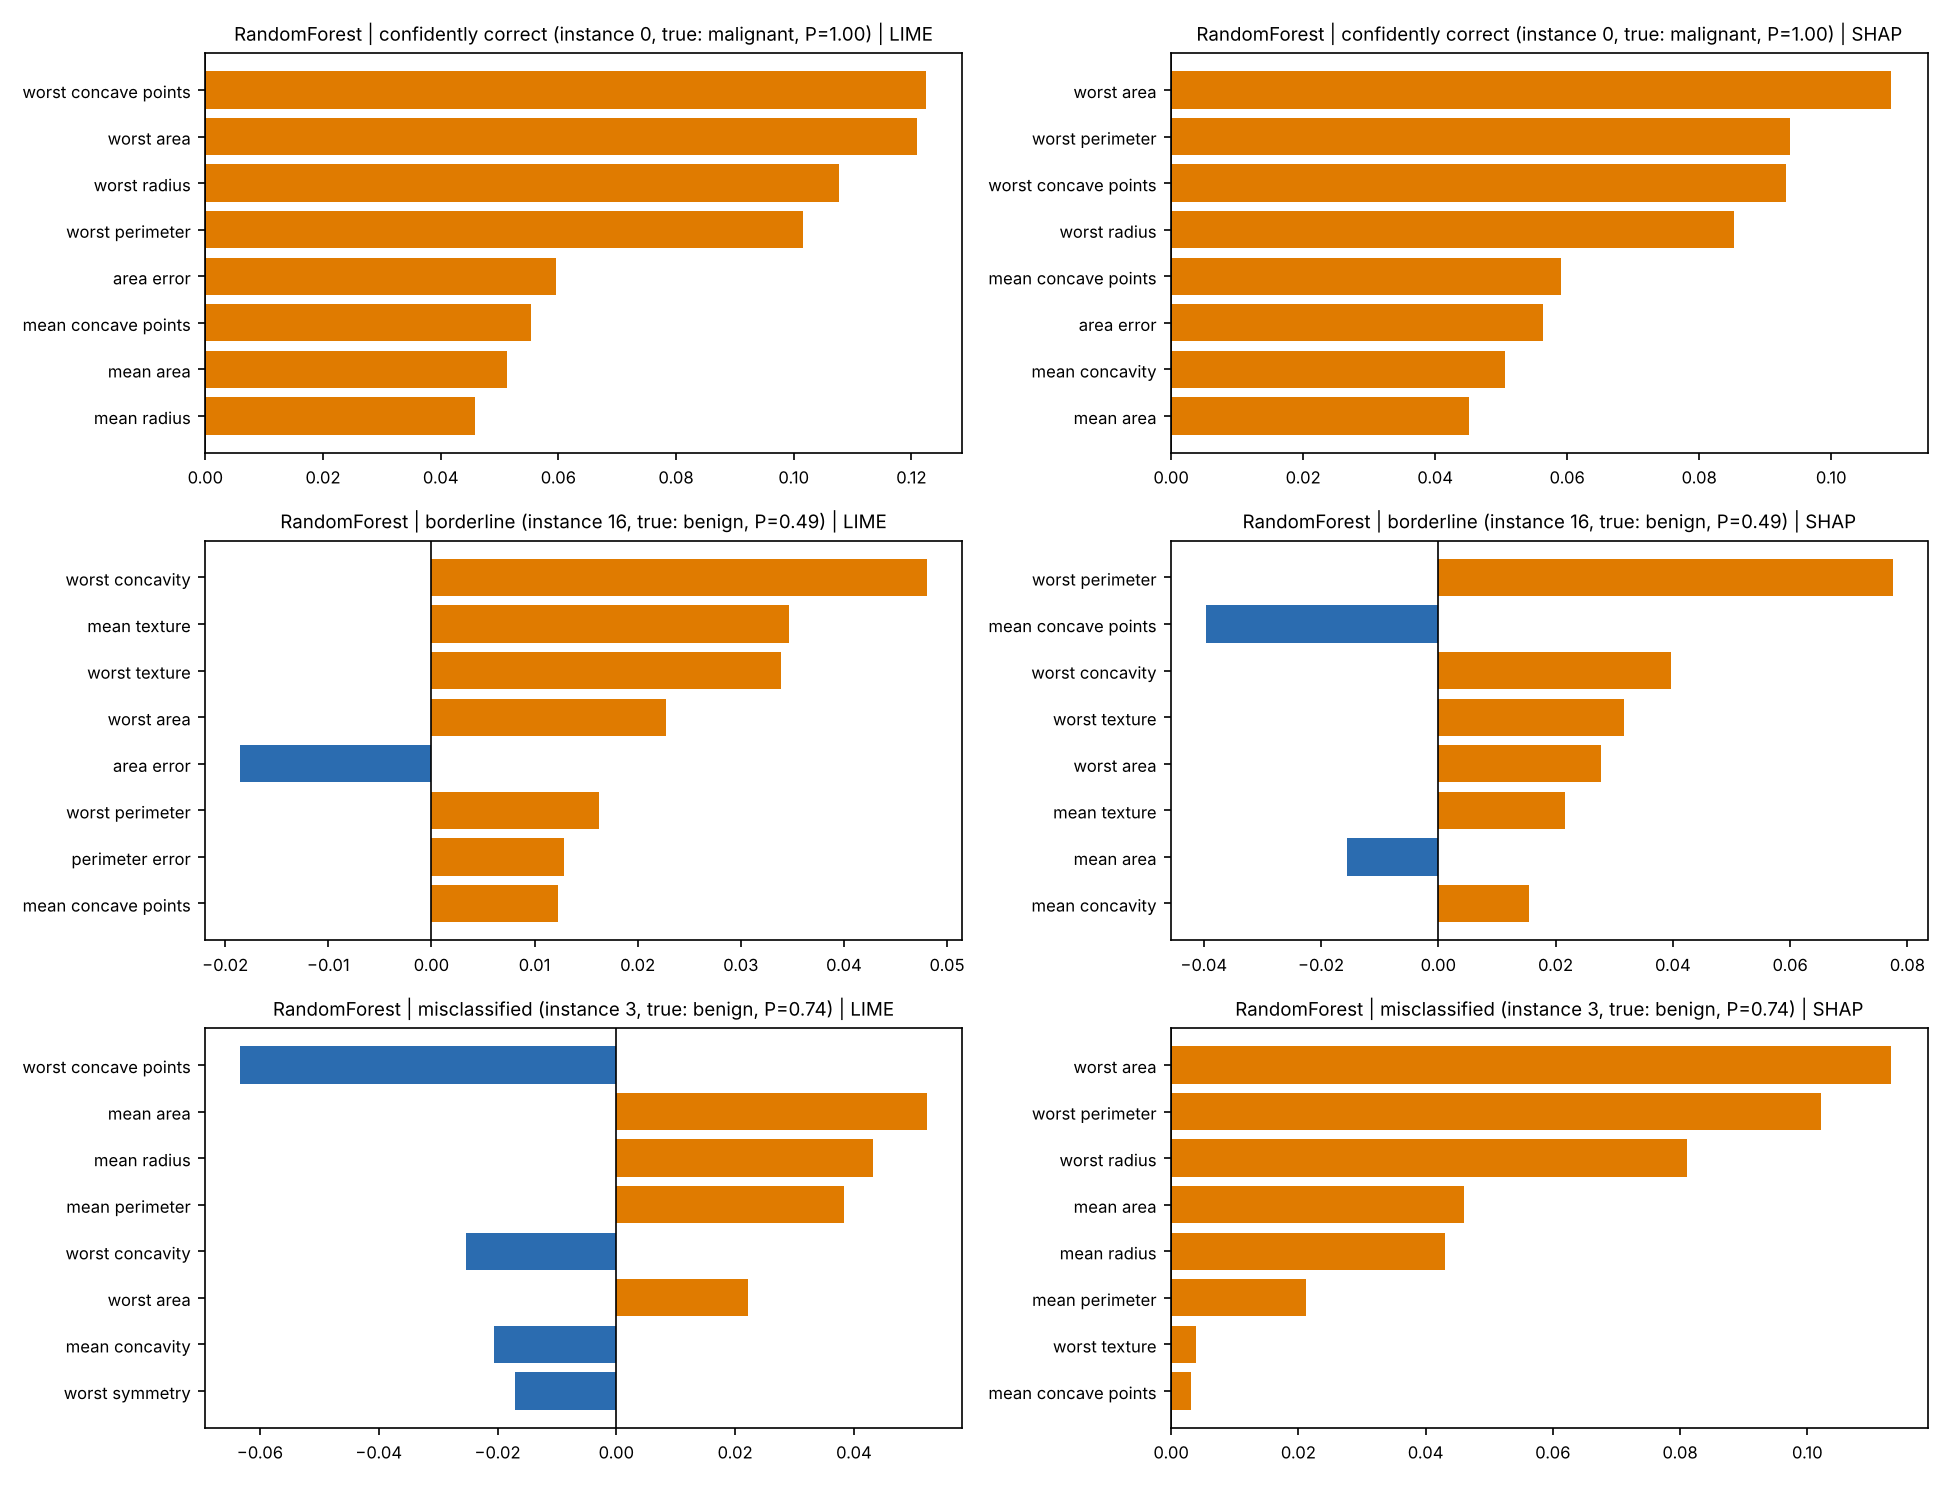
\includegraphics[width=\linewidth]{figs_en/contrib_RandomForest.png}
\caption{Feature contributions from LIME (left column) and SHAP (right column) for Random Forest; the three instances are, top to bottom, confidently correct, borderline and misclassified. Source: the team's experiment (\coderepo).}\label{fig:rf}
\end{minipage}\hfill
\begin{minipage}[t]{0.495\textwidth}
\centering
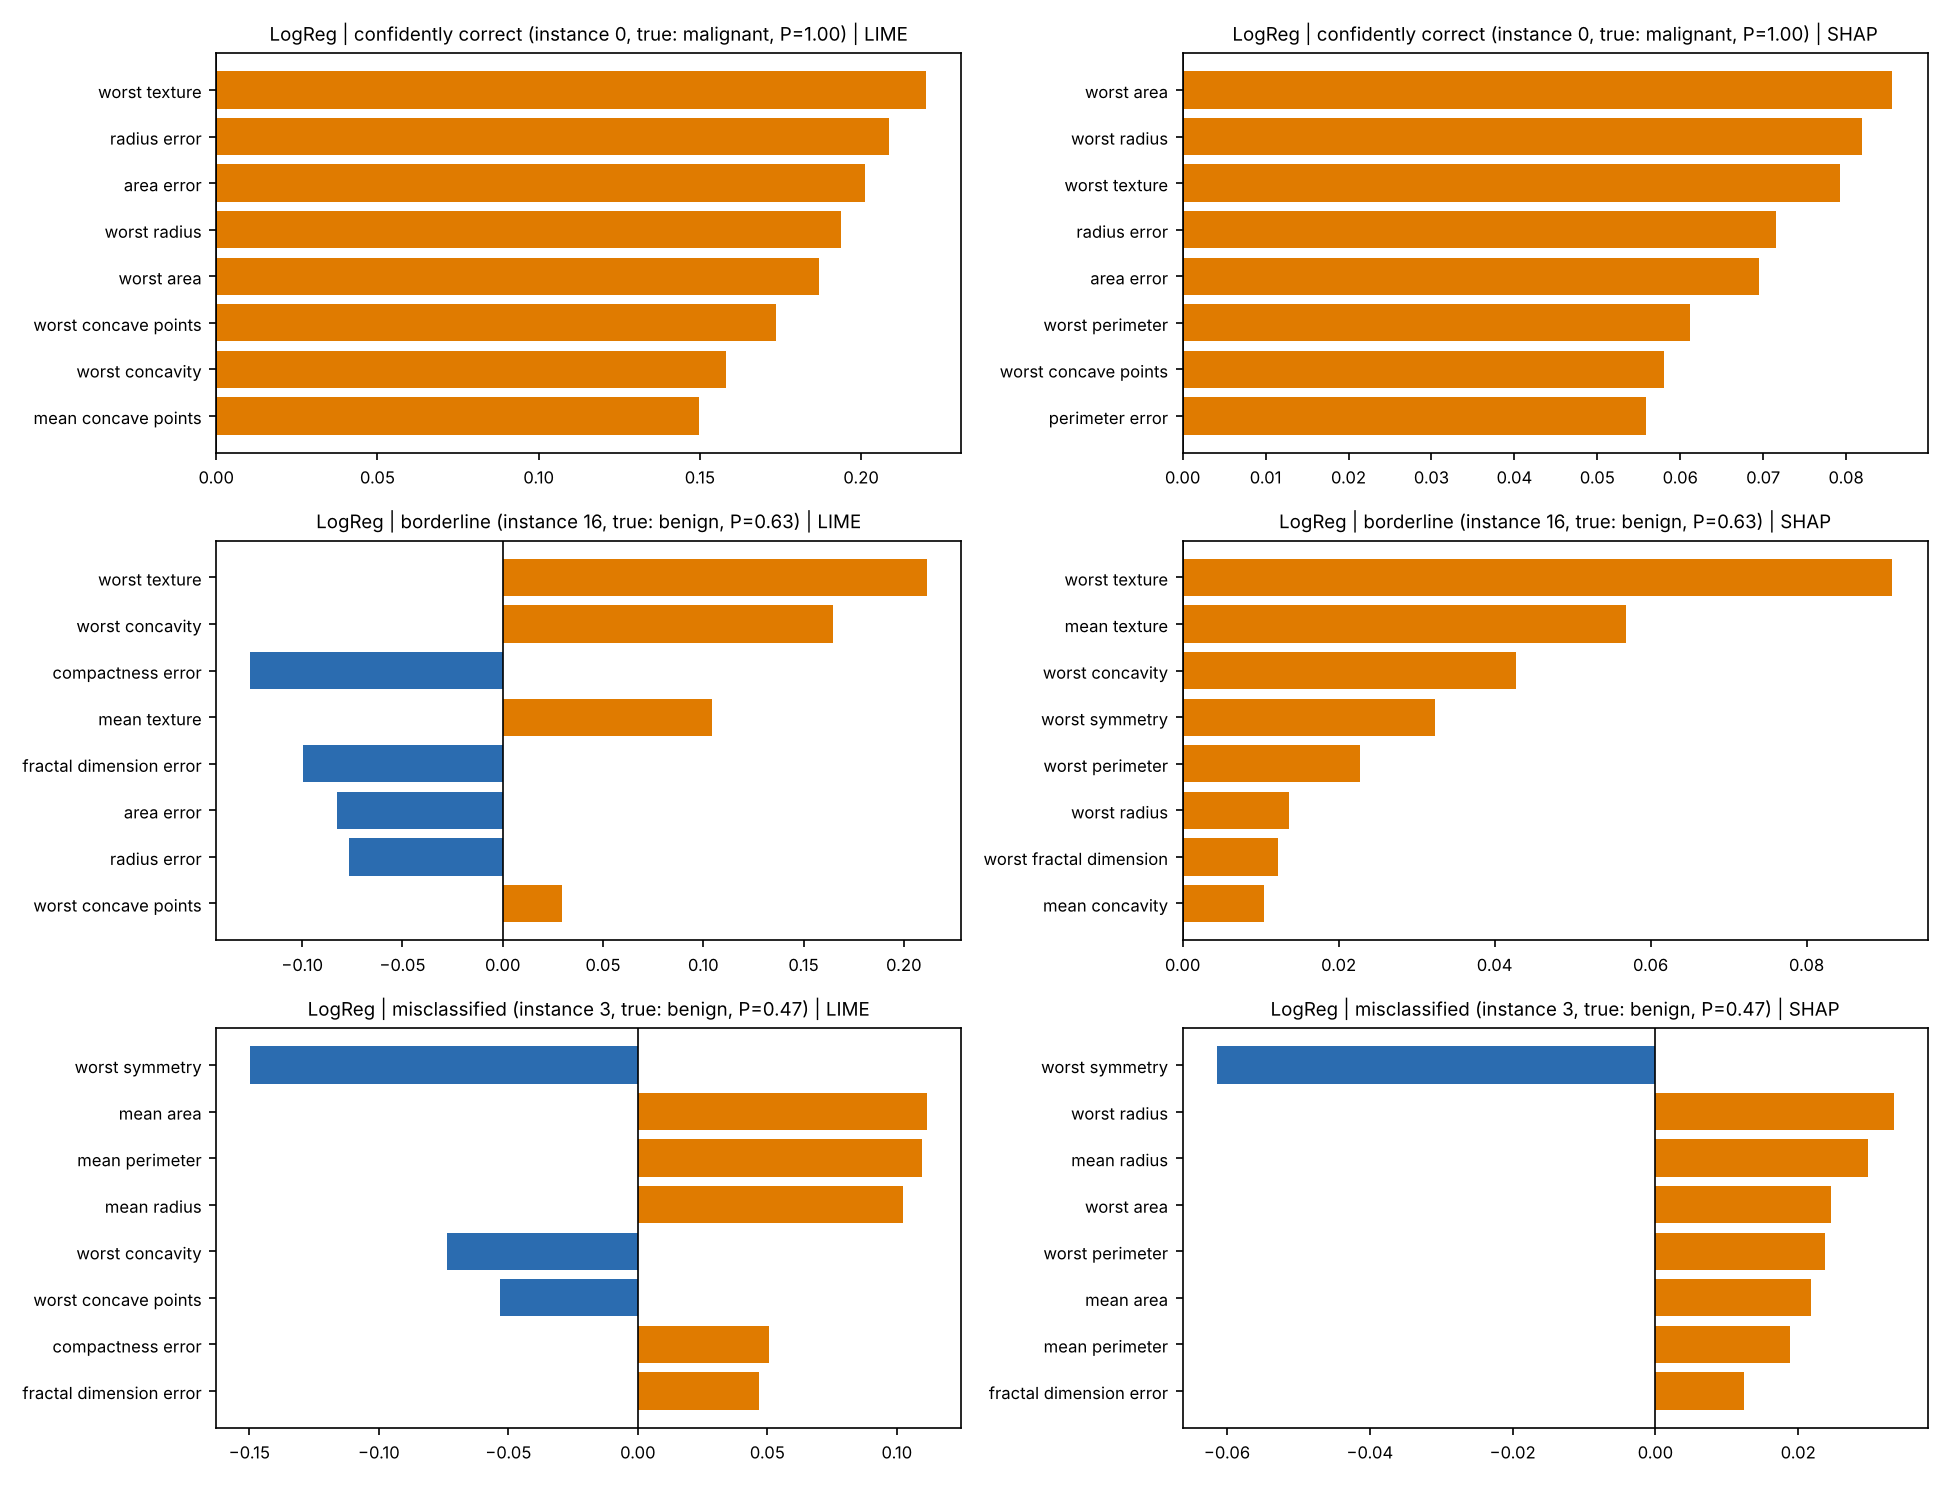
\includegraphics[width=\linewidth]{figs_en/contrib_LogReg.png}
\caption{Same as Figure~\ref{fig:rf} for Logistic Regression. On instance 3 Logistic Regression predicts correctly ($P = 0.466$). Source: the team's experiment (\coderepo).}\label{fig:lr}
\end{minipage}
\end{figure}

\subsection{LIME versus SHAP}
\label{sec:compare}
\emph{Overlap@5} is the number of features shared by the LIME and SHAP top-5
sets (ranked by $|\text{contribution}|$), divided by 5; it ranges from 0 (none
shared) to 1 (the same five, in any order). We report it for the main run and
as the average over all pairs of LIME and SHAP runs. \emph{Spearman's} $\rho
\in [-1, 1]$ compares how the two methods rank all 30 features by
$|\text{contribution}|$ ($-1$ reversed, 0 unrelated, 1 identical), so unlike
Overlap@5 it uses the order of every feature. We also record each method's top
feature and runtime (Table~\ref{tab:compare}).

\begin{table}[!htb]
\centering\footnotesize
\caption{LIME versus SHAP on the three instances. Overlap@5 is given as main
run / average over all run pairs; runtimes are given as LIME / SHAP.}\label{tab:compare}
\setlength{\tabcolsep}{3pt}
\begin{tabular}{@{}L{1.9cm}L{2.2cm}ccL{2.3cm}L{2.3cm}c@{}}
\toprule
\textbf{Model} & \textbf{Instance} & \textbf{Overlap@5} & \textbf{Spearman's $\rho$} & \textbf{Top-1 LIME} & \textbf{Top-1 SHAP} & \textbf{Runtime (s)}\\
\midrule
LogReg & Confidently correct & 1.0 / 0.80 & 0.74 & worst texture & worst area & 0.035 / 0.043\\
LogReg & Borderline & 0.6 / 0.67 & 0.24 & worst texture & worst texture & 0.037 / 0.035\\
LogReg & Misclassified & 0.4 / 0.49 & 0.26 & worst symmetry & worst symmetry & 0.040 / 0.034\\
Random Forest & Confidently correct & 0.8 / 0.82 & 0.83 & worst concave points & worst area & 0.066 / 0.441\\
Random Forest & Borderline & 0.6 / 0.71 & 0.69 & worst concavity & worst perimeter & 0.067 / 0.484\\
Random Forest & Misclassified & 0.4 / 0.44 & 0.46 & worst concave points & worst area & 0.069 / 0.390\\
\bottomrule
\end{tabular}
\end{table}

\textbf{Agreement falls as the instance gets harder.} For both models,
Overlap@5 drops from 0.8--1.0 on the confidently correct instance to 0.4 on
the misclassified one. When a feature appears in both top-5 sets, the two
methods always give it the same sign (sign agreement is 1.0 in all six cases).
The disagreement is therefore about \emph{which} features are selected, not
about the direction of their effect.

\textbf{Rankings differ most on the simplest model.} Spearman's $\rho$ is
lowest for Logistic Regression on the two hard instances (0.24 and 0.26), so
the full rankings differ substantially even for a linear model, and the top-5
sets overlap only in part (0.4--0.6). One possible, untested reason is that
LIME discretises continuous features by default.

\textbf{Runtime.} On Logistic Regression the two methods take about the same
time (about 0.04\,s). On Random Forest, KernelSHAP is about 6--7 times slower
than LIME (0.39--0.48\,s vs.\ about 0.07\,s), because it queries the model on
$2000$ coalitions $\times$ $100$ background instances. All timings come from a
single machine and varied by up to about 20\% between our runs.

\subsection{A case where the explanations disagree}\label{sec:wrong}
We now look in detail at the misclassified instance (test index 3), where the
Random Forest predicts $P(\text{malignant}) = 0.745$ although the true label is
benign. Table~\ref{tab:wrong} lists the top-5 features that each method gives
for this prediction. A positive contribution pushes the prediction towards
malignant, and a negative one pushes it towards benign.

\begin{table}[!htb]
\centering\small
\caption{Top-5 features of LIME and SHAP for the misclassified instance
(Random Forest, test index 3). Features shared by both methods are in bold.}\label{tab:wrong}
\begin{tabularx}{\textwidth}{L{1.9cm}XX}
\toprule
\textbf{Method} & \textbf{Top-5 by $|\text{contribution}|$} & \textbf{Signs}\\
\midrule
LIME & worst concave points, \textbf{mean area}, \textbf{mean radius}, mean perimeter, worst concavity & worst concave points and worst concavity negative; the rest positive\\
SHAP & worst area, worst perimeter, worst radius, \textbf{mean area}, \textbf{mean radius} & All positive\\
\bottomrule
\end{tabularx}
\end{table}

The two methods share only two features (mean area and mean radius), so
Overlap@5 is 0.4, and they tell different stories about the same prediction.
SHAP attributes the prediction almost entirely to size features, all of which
push towards malignant. LIME gives a mixed picture: its most important
feature, worst concave points, pushes towards benign, while several size
features push towards malignant.

No ground truth tells us which explanation is correct. One reading is that
the methods answer different questions: LIME asks which value ranges matter
near this instance, SHAP measures contributions relative to the average
prediction over the background data. Either way, two widely used methods
conflict on a wrong prediction, exactly where a user would rely on an
explanation, so explanations must be checked for faithfulness
(Section~\ref{sec:proc}).

\subsection{Stability}
\label{sec:stability}
An explanation is stable if running the method again with different random
choices gives a similar result. For LIME we vary the random seed (20 runs);
for SHAP we vary the background set (5 runs). We use two measures. The
\emph{Jaccard similarity} of two top-5 sets $A$ and $B$ is
$|A \cap B| / |A \cup B|$, and we report its mean over all pairs of runs; it
equals 1 when every run selects the same five features. Note that Jaccard is
stricter than Overlap@5: two sets sharing four of five features have Jaccard
$4/6 \approx 0.67$ but Overlap@5 $= 0.8$. \emph{Top-1 dominance} is the share
of runs in which the top-ranked feature is the one most often ranked first;
it equals 1 when every run agrees on the top feature.
Table~\ref{tab:stability} shows the results.

\begin{table}[!htb]
\centering\small
\caption{Stability of the top-5 features (LIME: 20 seeds; SHAP: 5 background sets).}\label{tab:stability}
\setlength{\tabcolsep}{4pt}
\begin{tabular}{llcccc}
\toprule
\textbf{Model} & \textbf{Instance} & \textbf{Jaccard LIME} & \textbf{Top-1 LIME} & \textbf{Jaccard SHAP} & \textbf{Top-1 SHAP}\\
\midrule
LogReg & Confidently correct & 0.78 & 0.95 & 0.68 & 0.40\\
LogReg & Borderline & 0.84 & 1.00 & 0.73 & 1.00\\
LogReg & Misclassified & 0.85 & 1.00 & 0.53 & 1.00\\
Random Forest & Confidently correct & 0.94 & 0.60 & 1.00 & 1.00\\
Random Forest & Borderline & 0.72 & 0.80 & 0.73 & 1.00\\
Random Forest & Misclassified & 0.74 & 1.00 & 1.00 & 1.00\\
\bottomrule
\end{tabular}
\end{table}

\textbf{Neither method is consistently more stable.} The mean Jaccard ranges
from 0.72 to 0.94 for LIME and from 0.53 to 1.00 for SHAP: SHAP is fully
stable on two RF instances, yet also has the lowest value in the table (LR,
misclassified instance).

\textbf{The top feature can change even on easy instances.} Top-1 dominance is
low in two cells: 0.60 for LIME on the Random Forest and 0.40 for SHAP on
Logistic Regression, both on the confidently correct instance. A possible
explanation, which we did not test, is that when $P$ is close to 1 many
features contribute similar amounts, so small changes are enough to swap the
top rank.

\textbf{An unstable example.} Figure~\ref{fig:unstable} shows how often each
feature enters the top-5 for the Random Forest on the borderline instance. Both
methods almost always include worst concavity, worst texture and worst
perimeter; they differ in ranks 4 and 5. LIME selects mean texture in 100\% of
runs and area error in 45\%, whereas SHAP selects mean concave points in 100\%
of runs (LIME only in 10\%) and mean texture in just 40\%. LIME's top feature
also changes between seeds: seed 0 ranks worst concavity first, while seeds
1--5 rank worst texture first.

\begin{figure}[!htb]
\centering
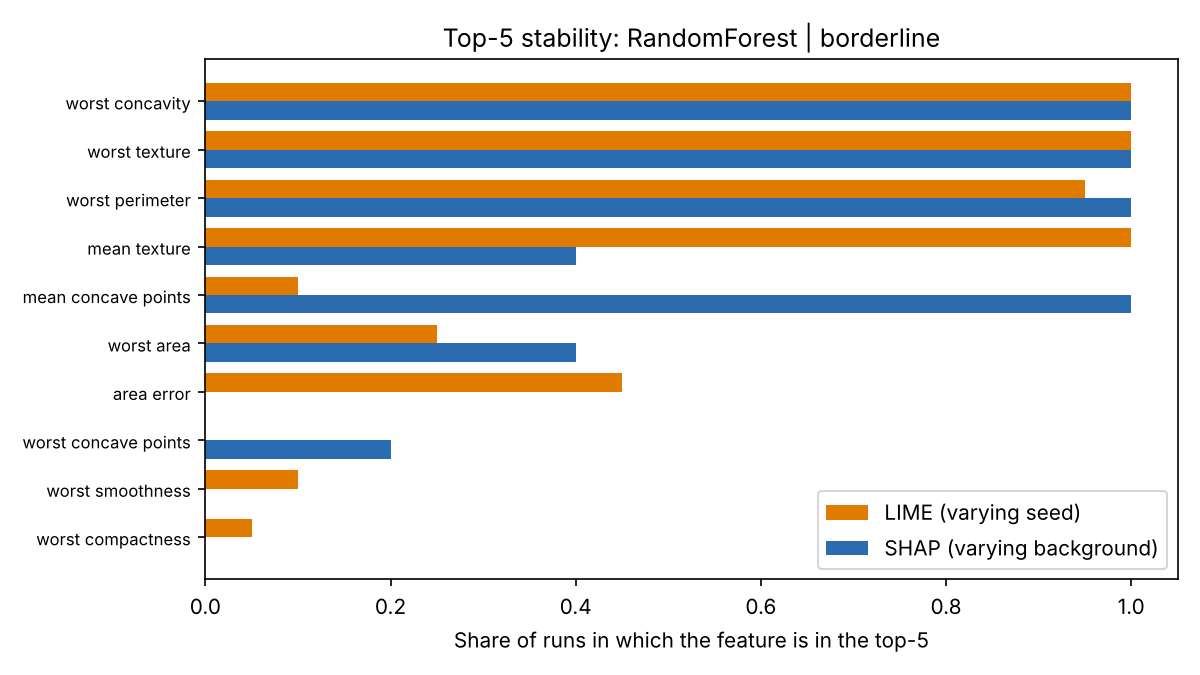
\includegraphics[width=0.6\textwidth]{figs_en/unstable_example.png}
\caption{Share of runs in which each feature appears in the top-5, Random
Forest, borderline instance (LIME: 20 seeds; SHAP: 5 background sets).
Source: the team's experiment (\coderepo).}\label{fig:unstable}
\end{figure}

\textbf{Tuning does not remove the instability.} Varying the SHAP background
size and the LIME kernel width on this instance (Appendix~\ref{app:sensitivity})
never lifts the Jaccard similarity above 0.73.

\subsection{Checking faithfulness with a deletion test}
\label{sec:deletion}
An explanation is faithful if the features it marks as important really drive
the model's prediction. We test this by deleting features and watching how the
prediction changes. For each of 20 randomly chosen test instances, we take the
features that the explanation says support the predicted class most strongly,
remove them one at a time (up to 10) by replacing each with its training-set
mean, and record the model's probability for the predicted class after each
removal. If the explanation is faithful, this probability should fall quickly.
As a baseline, we remove features in random order and average over 10 random
permutations. Figure~\ref{fig:del} shows the average curves.

\begin{figure}[!htb]
\centering\small
\pgfplotsset{delplot/.style={width=0.43\textwidth,height=4.6cm,xlabel={Features removed},xmin=0,xmax=10,ymin=0.5,ymax=1.0,
  xtick={0,2,4,6,8,10},grid=major,grid style={gray!25},tick label style={font=\scriptsize},label style={font=\footnotesize},
  title style={font=\footnotesize\bfseries},legend style={font=\scriptsize,at={(0.03,0.03)},anchor=south west,draw=none,fill=white,fill opacity=0.8},
  every axis plot/.append style={thick}}}
\begin{tikzpicture}
\begin{axis}[delplot,title={Random Forest},ylabel={Probability of predicted class}]
\addplot[color=orange!85!black,mark=*,mark size=1.5pt] coordinates {(0,0.923)(1,0.827)(2,0.777)(3,0.734)(4,0.717)(5,0.698)(6,0.674)(7,0.644)(8,0.629)(9,0.610)(10,0.605)};
\addplot[color=blue!70!black,mark=square*,mark size=1.5pt] coordinates {(0,0.923)(1,0.846)(2,0.776)(3,0.732)(4,0.701)(5,0.679)(6,0.651)(7,0.625)(8,0.602)(9,0.583)(10,0.563)};
\addplot[color=gray,dashed] coordinates {(0,0.923)(1,0.918)(2,0.909)(3,0.899)(4,0.888)(5,0.877)(6,0.869)(7,0.857)(8,0.847)(9,0.839)(10,0.830)};
\legend{LIME,SHAP,Random}
\end{axis}
\end{tikzpicture}\hfill
\begin{tikzpicture}
\begin{axis}[delplot,title={Logistic Regression}]
\addplot[color=orange!85!black,mark=*,mark size=1.5pt] coordinates {(0,0.941)(1,0.914)(2,0.892)(3,0.865)(4,0.836)(5,0.802)(6,0.753)(7,0.716)(8,0.675)(9,0.634)(10,0.579)};
\addplot[color=blue!70!black,mark=square*,mark size=1.5pt] coordinates {(0,0.941)(1,0.915)(2,0.889)(3,0.865)(4,0.836)(5,0.805)(6,0.774)(7,0.731)(8,0.693)(9,0.639)(10,0.584)};
\addplot[color=gray,dashed] coordinates {(0,0.941)(1,0.940)(2,0.937)(3,0.938)(4,0.937)(5,0.934)(6,0.933)(7,0.929)(8,0.927)(9,0.925)(10,0.923)};
\legend{LIME,SHAP,Random}
\end{axis}
\end{tikzpicture}
\caption{Deletion test: average probability of the predicted class as the
top-ranked features are removed (20 test instances, one seed). A faster drop
means a more faithful explanation. Source: the team's
\code{results/deletion\_curves.csv} (\coderepo).}\label{fig:del}
\end{figure}

Both LIME and SHAP lower the probability much faster than random removal. After 5 removals, Random Forest falls from 0.923 to 0.698 (LIME) and 0.679 (SHAP) but only to 0.877 at random; Logistic Regression falls from 0.941 to 0.802, 0.805 and 0.934. LIME and SHAP differ by at most 0.02 at 5 features and by 0.04 at 10 (RF: 0.605 vs.\ 0.563), which, with one seed, 20 instances and no confidence intervals, is not enough to rank them. Caveats: mean replacement can create out-of-distribution samples, and with strongly correlated features removing one does not remove its information.

\subsection{Feature importance is not a causal effect}
\label{sec:causal}
LIME and SHAP describe how the \emph{model} uses its features, not how those
features affect the \emph{disease}: a large contribution means the model
relies on a feature, not that it causes malignancy. Four reasons, each visible in our experiment, show why the two should not be confused.

\begin{itemize}
  \item \textbf{Correlated features.} Worst radius, perimeter and area grow
        together and all appear near the top of the charts; how the credit is
        split among them depends on the model and the background data, not on
        which one is the real cause.
  \item \textbf{Unrealistic samples.} Both LIME and KernelSHAP change each feature 
        independently of the others; for KernelSHAP this is the feature-independence 
        assumption described in Section~\ref{sec:shap}. This creates combinations that never occur 
        in real tumours, such as a large area with a small radius, so the model is 
        queried in regions where it has never seen data.
  \item \textbf{Explanations also reflect the model's mistakes.} On the
        misclassified instance (Section~\ref{sec:wrong}) the size features
        explain why the model erred, not that the tumour is malignant.
  \item \textbf{Replacing a value is not a real intervention.} It is a
        computation on the model; knowing what would happen if tumour size
        actually changed requires causal assumptions that neither method tests.
\end{itemize}
Conclusions should therefore be phrased as ``the model relies on $X$'', not as
``$X$ causes $Y$''.

\subsection{A procedure for evaluating faithfulness (proposed)}\label{sec:proc}
Since LIME and SHAP can disagree and change between runs, we propose the
five-step procedure below, organised (in spirit, not by its exact formulas)
around the criteria of Mersha et al.~\cite{mersha}. Each step names its
criterion and whether we carried it out.

\begin{enumerate}
  \item \textbf{Sanity check with a known answer} (fidelity). For a linear
        model, the explanation must match $w_j (x_j - \mu_j)$. \emph{Status:}
        done on the worked example (Section~\ref{sec:shaphand}), not yet on
        the experiment's LR.
  \item \textbf{Local fit} (fidelity). LIME: weighted $R^2$ of the surrogate
        around $x$; SHAP: $\varphi_0 + \sum_j \varphi_j = f(x)$.
        \emph{Status:} SHAP checked (Section~\ref{sec:charts}); LIME $R^2$
        not computed.
  \item \textbf{Deletion and insertion vs.\ random order} (fidelity,
        sufficiency). \emph{Status:} deletion done
        (Section~\ref{sec:deletion}); insertion not done.
  \item \textbf{Stability} (consistency). Top-$k$ Jaccard and its variance
        over many seeds and background sets. \emph{Status:} done
        (Section~\ref{sec:stability}, Appendix~\ref{app:sensitivity}).
  \item \textbf{Robustness.} Change in the explanation under small input
        perturbations or across models of similar accuracy.
        \emph{Status:} not done.
\end{enumerate}

Efficiency is measured by runtime (Section~\ref{sec:compare}). An explanation
should be considered reliable only if it passes several of these checks
together; passing a single one is not enough.

%---------------------------------------------------------------------
\section{Conclusion}
Our answer to the guiding question is no: a highly accurate prediction does
not necessarily come with a reliable explanation. Although the two models
reach 98.2\% and 95.6\% test accuracy, LIME and SHAP share only two of their
five most important features on the misclassified instance (Overlap@5 $=0.4$).
Each method's top-5 also changes between runs, with a mean Jaccard similarity
as low as 0.53 for SHAP and 0.72 for LIME. In the deletion test, both methods
find influential features far better than a random order, but neither is
shown to be more faithful, and neither reveals causal relationships.

\textbf{Conditions of use.} An explanation describes the model's behaviour,
either around one instance (LIME) or relative to a baseline (SHAP). Users
should report the seed, background data and kernel width, repeat the
explanation and report its stability, and apply the checks of
Section~\ref{sec:proc}, above all for borderline and misclassified instances.

\textbf{Limitations and future work.} With one dataset, three instances, two
models and no confidence intervals, the conclusions are illustrative
(Appendix~\ref{app:limits}). Next steps are the insertion test, the LIME
$R^2$, TreeSHAP, the log-odds scale, more datasets and more repetitions.

%---------------------------------------------------------------------
\begin{thebibliography}{9}
\bibitem{ribeiro} Ribeiro, M. T., Singh, S., \& Guestrin, C. (2016). ``Why Should I Trust You?'': Explaining the Predictions of Any Classifier. \emph{KDD 2016}, 1135--1144. \href{https://doi.org/10.1145/2939672.2939778}{DOI}.
\bibitem{mersha} Mersha, M., Lam, K., Wood, J., AlShami, A., \& Kalita, J. (2024). Explainable artificial intelligence: A survey of needs, techniques, applications, and future direction. \emph{Neurocomputing}, 599, 128111. \href{https://doi.org/10.1016/j.neucom.2024.128111}{DOI} (we read the arXiv version 2409.00265v2).
\bibitem{lundberg} Lundberg, S. M., \& Lee, S.-I. (2017). A Unified Approach to Interpreting Model Predictions. \emph{NeurIPS 2017}. \href{https://proceedings.neurips.cc/paper_files/paper/2017/hash/8a20a8621978632d76c43dfd28b67767-Abstract.html}{Paper page}.
\bibitem{street} Street, W. N., Wolberg, W. H., \& Mangasarian, O. L. (1993). Nuclear feature extraction for breast tumor diagnosis. \emph{IS\&T/SPIE 1993 International Symposium on Electronic Imaging: Science and Technology}, vol.\ 1905, 861--870. \href{https://api.semanticscholar.org/CorpusID:14922543}{Paper page}.
\end{thebibliography}

\section*{Data, tools and source of the numbers}
\begin{itemize}
  \item \textbf{Data.} Breast Cancer Wisconsin (Diagnostic) \cite{street},
        loaded with\\ \code{sklearn.datasets.load\_breast\_cancer}.
  \item \textbf{Software.} Python with the scikit-learn, \code{lime} and
        \code{shap} libraries.
  \item \textbf{Source of the numbers.} All figures, tables, numbers and both
        worked examples were produced by the team with the notebook
        \code{S04\_LIME\_SHAP\_}\allowbreak\code{experiments.ipynb}; none are
        taken from the cited papers.
  \item \textbf{Use of AI tools.} Claude (Anthropic) was used to help explain
        concepts, write the experiment code, and draft and revise this report.
  \item \textbf{Verification of AI-assisted content.} We checked every claim
        about LIME and SHAP against the original papers
        \cite{ribeiro}\cite{lundberg} and the survey \cite{mersha}; re-ran the
        notebook and compared every number in the tables and text with the
        CSV files in \code{results/}; and recomputed both worked examples
        independently (by hand and with a short NumPy script).
  \item \textbf{Code repository.} The notebook and all results of our experiments are available at
\url{https://github.com/khoiLearnsToCode/CS420_AI_LIME_SHAP}.
\end{itemize}

%---------------------------------------------------------------------
\appendix
\section{Full experimental setup}\label{app:setup}

\begin{table}[!htb]
\centering\small
\caption{Experimental setup.}\label{tab:setup}
\begin{tabularx}{\textwidth}{L{2.4cm}XL{3.8cm}}
\toprule
\textbf{Component} & \textbf{Choice} & \textbf{Reason}\\
\midrule
Data & Breast Cancer Wisconsin \cite{street}, loaded from scikit-learn: 569 instances, 30 features, class 0 = malignant, class 1 = benign; 80/20 stratified split with \code{random\_state = 42} (455 train, 114 test) & Public, binary and readily available\\
Models & Logistic Regression (with standardisation) and a 200-tree Random Forest; test accuracy 98.2\% and 95.6\% & A linear model as a reference and a less transparent model to expose instability\\
Explanation space & Probability $P(\text{malignant})$ & LIME explains predicted probabilities \cite{ribeiro}, so this makes the two methods directly comparable. As a result, the $\varphi$ values add up on the probability scale, not on the log-odds scale\\
SHAP & KernelSHAP \cite{lundberg} with 100 background instances drawn from the training set and 2000 sampled coalitions & The same model-agnostic tool for both models, so runtimes are comparable\\
LIME & 5000 perturbed samples, default kernel width $0.75\sqrt{d} \approx 4.11$, default discretisation & The library's standard configuration\\
Three instances & A fixed rule applied to the RF: the correct prediction with the highest confidence (index 0), the prediction with the smallest $|P - 0.5|$ (index 16) and the first misclassified instance (index 3) & Prevents selecting favourable examples\\
Number of runs & LIME: 20 seeds; SHAP: 5 background sets (seeds 0--4); top-$k$ with $k = 5$ & A compromise between measuring stability and keeping runtime low\\
Deletion test & 20 random test instances (fixed seed); up to 10 features removed by replacing them with the training mean & Checks faithfulness\\
\bottomrule
\end{tabularx}
\end{table}

\section{Sensitivity to background size and kernel width}\label{app:sensitivity}
Section~\ref{sec:stability} showed that the explanations change between runs.
Here we check whether this instability can be reduced by changing the main
parameter of each method: the size of the background set for SHAP and the
kernel width for LIME. We use the Random Forest on the borderline instance,
the case where LIME is least stable (Jaccard 0.72) and SHAP is also not fully stable (0.73). For each background size
we run SHAP on 5 background sets, and for each kernel width we run LIME with
10 seeds. Because LIME uses fewer seeds here than the 20 of
Section~\ref{sec:stability}, its Jaccard values are not directly comparable
with Table~\ref{tab:stability}. Table~\ref{tab:sensitivity} shows the results.

\begin{table}[!htb]
\centering\small
\caption{Sensitivity to parameters (Random Forest, borderline instance).}\label{tab:sensitivity}
\begin{tabular}{llcc}
\toprule
\textbf{Method} & \textbf{Parameter} & \textbf{Jaccard top-5} & \textbf{Top-1 dominance}\\
\midrule
SHAP & background = 10 & 0.63 & 0.8\\
SHAP & background = 50 & 0.73 & 1.0\\
SHAP & background = 100 (default) & 0.73 & 1.0\\
LIME & kernel width = 1.00 & 0.65 & 0.7\\
LIME & kernel width = 2.00 & 0.68 & 0.9\\
LIME & kernel width = 4.11 (default) & 0.68 & 0.9\\
LIME & kernel width = 8.00 & 0.68 & 0.9\\
\bottomrule
\end{tabular}
\end{table}

For SHAP, a background of only 10 instances lowers stability (Jaccard 0.63),
but increasing it beyond 50 brings no further gain (0.73). For LIME, a small
kernel width of 1.0 is slightly less stable (0.65), and all widths from 2.0
upwards give the same result (0.68). Even the best settings stay well below 1,
so tuning these parameters does not remove the instability on this instance.

\section{Limitations}\label{app:limits}
\begin{itemize}
  \item Only one dataset, three instances and two models; the results may not generalise.
  \item 20 seeds (LIME) and 5 background sets (SHAP) are few, and there are no confidence intervals.
  \item The deletion test uses one seed and 20 instances, and replacing with the mean can create out-of-distribution samples.
  \item Runtimes are from one machine and for KernelSHAP; TreeSHAP for Random Forest would be much faster (not measured).
  \item Explanations are on the probability scale; on log-odds the results may differ (not tested).
  \item LIME discretises features, so only ranks and signs can be compared with SHAP, not absolute magnitudes.
  \item There is no ground truth for the Random Forest's explanations, so we cannot say which method is ``correct''.
\end{itemize}

\end{document}
